%!TEX root = mainfile.tex

\section{Observational Gravitational Lensing} % (fold)
\label{sec:observational_gravitational_lensing}
	The phenomenon of gravitational lensing has the potential to be very useful for the chosen observing strategy. Lensing will allow distant objects that could not otherwise have been seen to be observed and identified.  This could be a very important part of the observing strategy as we look to push boundaries to observe objects at as yet unexplored redshifts. There is a trade-off when using gravitational lenses between the ability to see to much higher redshifts using the magnification and the fact that the viewing area is decreased due to obscuration by the lens and the increased size of the images. As a result, the most useful way to integrate gravitational lensing into the strategy will be to use it as a supplement to the deep survey, to attempt to observe a few objects at very high redshift, rather than to magnify and better resolve sources that can be detected otherwise.

	There are two routes that can be taken to select a lens: either known lenses from surveys that have already been carried out can be used, or a new set of lenses can be located as part of the observing strategy. Examples of surveys that have been carried out previously include Cluster Lens And Supernova survey with Hubble (CLASH)\cite{CLASH} and the MAssive Cluster Survey (MACS)\cite{MACS}. There are only a limited number of massive clusters known, and a disadvantage of selecting those from other surveys is that they may already have been studied, for example, CLASH has already located a candidate $z\approx11$ galaxy behind cluster MACSJ0647.7+7015\cite{CLASH_z11_candidate}. The chances of located strongly lensed high redshift galaxies will be greater if new lenses are selected. There are several advantages to using clusters that have already been found, for example, many of them will have masses and velocity dispersions that have been well determined, allowing an accurate calculation of the magnification to be made. It may also reduce the observing time for the strategy if an extra survey must be made to find the lenses.

	The second option, to locate new clusters, is appealing because the lenses chosen can be carefully selected with optimum properties for the observing strategy. Both CLASH and MACS used x-ray emission selection criteria in order to find a range of cluster masses, however for the purposes of this strategy, selection using the strong lensing properties of the cluster would be the best option. The stronger the lensing exhibited by a cluster, the more useful it is likely to be for observing very faint objects. The region of sky in which the lenses lie can be chosen such that it is compatible with all the telescopes chosen for the observing strategy. By selecting based on lensing properties, it is likely that the lenses chosen will be very massive since the lensing strength depends directly on lens mass, as shown in figure~\ref{fig:Lensing_cross_section_as_a_function_of_mass}\cite{Optimal_mass_configurations}.
	\begin{figure}[!htb]
		\centering
			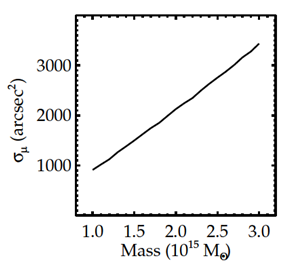
\includegraphics[width=0.4\textwidth]{../Images/Lensing_cross_section_as_a_function_of_mass.png}
		\caption[Lensing cross section as a function of mass]{\cite{Optimal_mass_configurations}Plot of the lensing cross section as a function of mass for a spherical halo at z=0.5. The dependence of cross section on mass can be clearly seen, indicating that the more massive a cluster, the better a lens it will be.\label{fig:Lensing_cross_section_as_a_function_of_mass}}
	\end{figure}

	The lens redshift also has a significant effect on the magnification of the source. As a result, it is important to choose a range of redshifts within which the lenses found must lie. The shear caused by a lens at a given redshift is given by
	\begin{align}
		\gamma(r) &= \frac{4\pi G}{c^2}\frac{D_{LS}D_{L}}{D_S}\left( \overline{\Sigma}(<r)-\Sigma(r) \right)
	\end{align}

	where $\overline{\Sigma}(<r)$ is the mean projected surface mass density within r and $\Sigma(r)$ the projected surface mass density at $r$. Keeping the radius (and therefore surface mass density) constant, figure~\ref{fig:shear_as_a_function_of_source_redshift} shows the dependence of shear on source redshift at fixed lens redshifts. The point at which each curve crosses the x-axis is the lens redshift, since the magnification is equal to 0 at the lens. It can be seen from the plot, that at low source redshifts, the shear distortion is immeasurably small. As the redshift increases to around 0.5, the lower redshift clusters will distort the source images. Once the source redshift is greater than 1, shear distortion is seen around all the lenses\cite{Constraining_source_redshift_distributions}.
	\begin{figure}[!htb]
		\centering
			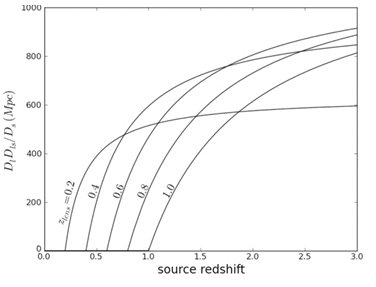
\includegraphics[width=0.5\textwidth]{../Images/Shear_as_a_function_of_source_redshift.png}
		\caption[Shear as a function of source redshift]{\cite{Constraining_source_redshift_distributions}A plot of shear against source redshift, with each line representing a different lens redshift. The point at which the lines cross the x-axis is the lens redshift, since at the lens, the magnification of the source is equal to 0.\label{fig:shear_as_a_function_of_source_redshift}}
	\end{figure}

	A similar plot is shown in figure [Einstein angle as a function of source redshift], but in this case, the relation between source redshift and Einstein angle is seen. From this plot, the Einstein angle and hence the strength of the lens decreases as the lens redshift increases, with the Einstein angle increasing rapidly for source redshifts just past that of the lens, and then rapidly saturating.
	\begin{figure}[!htb]
		\centering
			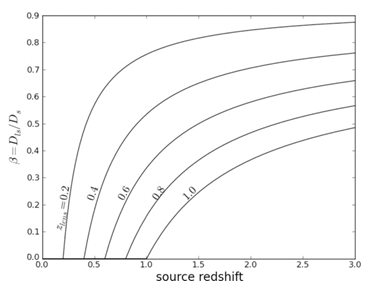
\includegraphics[width=0.5\textwidth]{../Images/Einstein_angle_as_a_function_of_source_redshift.png}
		\caption[Einstein angle as a function of source redshift]{\cite{Constraining_source_redshift_distributions} Plot of Einstein angle against source redshift. Again, each line corresponds to a different lens redshift. The point at which each line crosses the x-axis is the lens redshift, since at the lens, the magnification of the source is equal to 0.\label{fig:Einstein_angle_as_a_function_of_source_redshift}}
	\end{figure}

	Combining these two results, the optimum lens redshift is found to be around 0.6. A range of lens redshifts within which the lenses chosen must lie will be defined.

	The magnification of the source can be roughly calculated using the arcs formed by the images. The Einstein radius can be approximated by taking the mean distance from the centre of the lens to the two images. For strong lensing to occur, it is a mathematical requirement for the projected surface density to be greater than the critical surface density which is given by\cite{Critical_surface_density}
	\begin{align}
		\Sigma_c &= \frac{c^2}{4\pi G}\frac{D_L}{D_L D_{LS}}
	\end{align}
	Assuming that Einstein radius encloses the significant mass, an estimate of the mass can be made from
	\begin{align}
		M &= \Sigma_c \pi \theta_E^2
	\end{align}
	since the thin lens approximation is being used. Similarly, an order of magnitude calculation of the magnification can be made using
	\begin{align}
		\mu &= \frac{x_E}{x_E -1}
	\end{align}
	where $x_E$ is the radial co-ordinate in units of the Einstein radius\cite{Lens_mass_estimate}.
% section observational_gravitational_lensing (end)
